\documentclass[10pt,a4paper]{article}
\usepackage[margin=0.82in]{geometry}
\usepackage{amsmath,amssymb,booktabs,graphicx,microtype,hyperref,array,float}
\graphicspath{{figures/}}
\hypersetup{colorlinks=true,linkcolor=black,citecolor=blue,urlcolor=blue}
\newcommand{\um}{\ensuremath{\mu\mathrm{m}}}
\newcommand{\wn}{\ensuremath{\mathrm{cm}^{-1}}}
\title{Dual-Angle FTIR Measurement of a SiC Epitaxial-Layer Thickness:\\Evidence for a 7.4--7.6 \um\ Candidate Interval}
\author{Cai Wenjie\\Xiamen University\\\href{mailto:19020232202343@stu.xmu.edu.cn}{19020232202343@stu.xmu.edu.cn}}
\date{}
\begin{document}
\maketitle
\begin{abstract}
Thickness is a defining geometrical parameter of a SiC epitaxial layer, but an infrared fringe period is not itself a calibrated thickness when complex refractive response, multiple reflection and instrument response are uncertain. We analyse FTIR reflectance from one SiC epi-wafer acquired at incidence angles of $10^\circ$ and $15^\circ$. The primary measurement conclusion is a candidate thickness interval of \textbf{7.4--7.6 \um}. A constrained dual-angle transfer-matrix inversion has a representative minimum of $7.465\,\um$ (joint RMSE $0.00171152$), but this value is not presented as independently certified ground truth. The evidence is ordered deliberately. Multiple detrending routes and sliding-window Fourier analysis find a stable interference period near $250\,\wn$ ($244.537$--$256.000\,\wn$), establishing phase information. Fringe-order-difference estimates vary substantially with the refractive-index convention, showing why phase alone is insufficient. A bounded Lorentz--Drude optical response, one shared thickness, and angle-specific affine terms profiled from the nonlinear search then provide the physical mapping. Four band-weight schemes shift the local minimum by at most $0.020\,\um$; fixed-material profile and moving-block bootstrap checks support local stability. However, the $15^\circ$ residual is larger and highly autocorrelated, and an epitaxial plasma-scale parameter reaches its bound. The result is therefore an internally supported thickness measurement statement, not an accuracy claim: independent profilometry, cross-sectional SEM or ellipsometry is required to validate absolute error and full physical uncertainty.
\par\noindent\textbf{Keywords:} 4H--SiC; epitaxial layer; FTIR reflectance; thickness measurement; transfer matrix; identifiability
\end{abstract}

\section{Measurement question and evidence standard}
SiC power devices depend on the geometry of their epitaxial drift layers, making layer thickness an important manufacturing quantity. Infrared reflectance offers a non-contact route because repeated reflections between the air--epilayer and epilayer--substrate interfaces generate interference structure. Earlier SiC work has used fringe-order differences and FTIR reflectance for thickness determination \cite{Li2010,Tang2009,Dong2012}. The physical attraction of this route does not remove its inverse-problem difficulty: the observed phase combines thickness with dispersion, absorption, interface contrast, angle and the measurement chain. General thin-film transfer-matrix formalisms make this dependence explicit \cite{Troparevsky2010}.

The question addressed here is narrow: what thickness statement is justified by the two recorded FTIR spectra of this wafer? Four evidence levels are kept distinct. First, spectral periodicity establishes that the data contain a repeatable phase scale. Second, a bounded optical model maps that scale to candidate thickness. Third, profile, resampling and weight perturbations test local stability within that model. Fourth, external metrology would be required to establish absolute accuracy. Conflating these levels is the principal route by which a numerically sharp fit becomes an over-precise measurement claim.

\begin{figure}[H]\centering
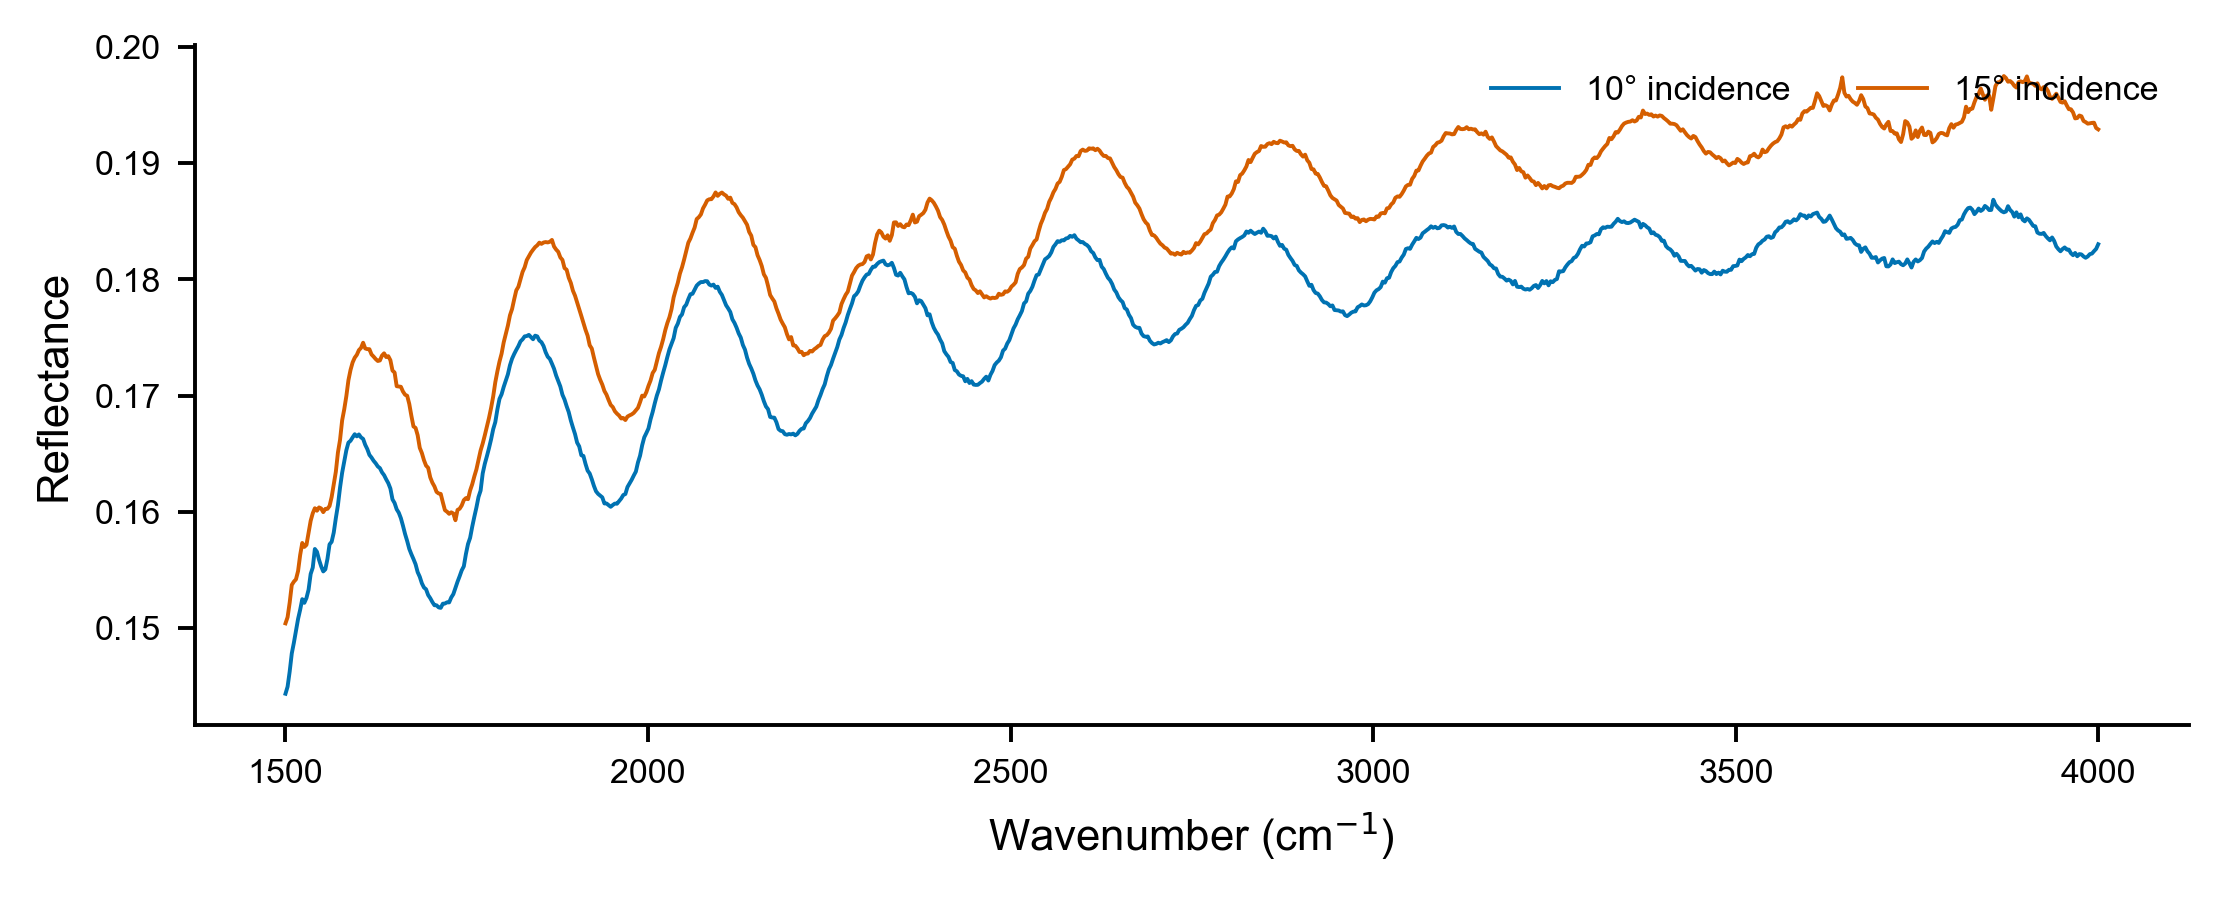
\includegraphics[width=.94\linewidth]{en_raw_dual_angle.png}
\caption{Recorded dual-angle SiC reflectance spectra. Oscillations motivate phase-based inversion, whereas their changing envelope and angle dependence rule out treating the spectra as ideal sinusoids.}\label{fig:raw}
\end{figure}

\section{Data, optical model and inference design}
\subsection{Recorded observations and analysis scope}
The data consist of normalised FTIR reflectance spectra from one SiC epi-wafer measured at $10^\circ$ and $15^\circ$. Each original workbook contains 7,469 wavenumber--reflectance pairs. The primary analysis uses $1500$--$4000\,\wn$: it retains several visible interference oscillations while avoiding the interpretation of difficult low-wavenumber structure as direct thickness evidence. No profilometer, ellipsometric, cross-sectional SEM, or certified-reference thickness is available. Thus the data support internal consistency analysis, not a direct calculation of metrological error.

The inference makes its geometrical and processing assumptions explicit. The epilayer/substrate interfaces are treated as locally parallel, so both angles share one scalar thickness; the two spectra are treated as measurements of the same wafer; and sufficient optical contrast is assumed for the layer to be identifiable. FFT and FOD are restricted to phase-scale diagnosis and basin construction, whereas the TMM supplies the primary thickness statement. Raw spectra were sorted in wavenumber, normalised to fractional reflectance and interpolated onto a uniform wavenumber grid before Fourier analysis. Centring, moving-average, low-order-polynomial, rolling-baseline and first-difference preprocessing were used only to test persistence of the periodic signal, not as freely tuned components of the physical fit. Sliding windows of width $1200\,\wn$ and step $250\,\wn$ give periods from $244.537$ to $256.000\,\wn$.

\begin{figure}[H]\centering
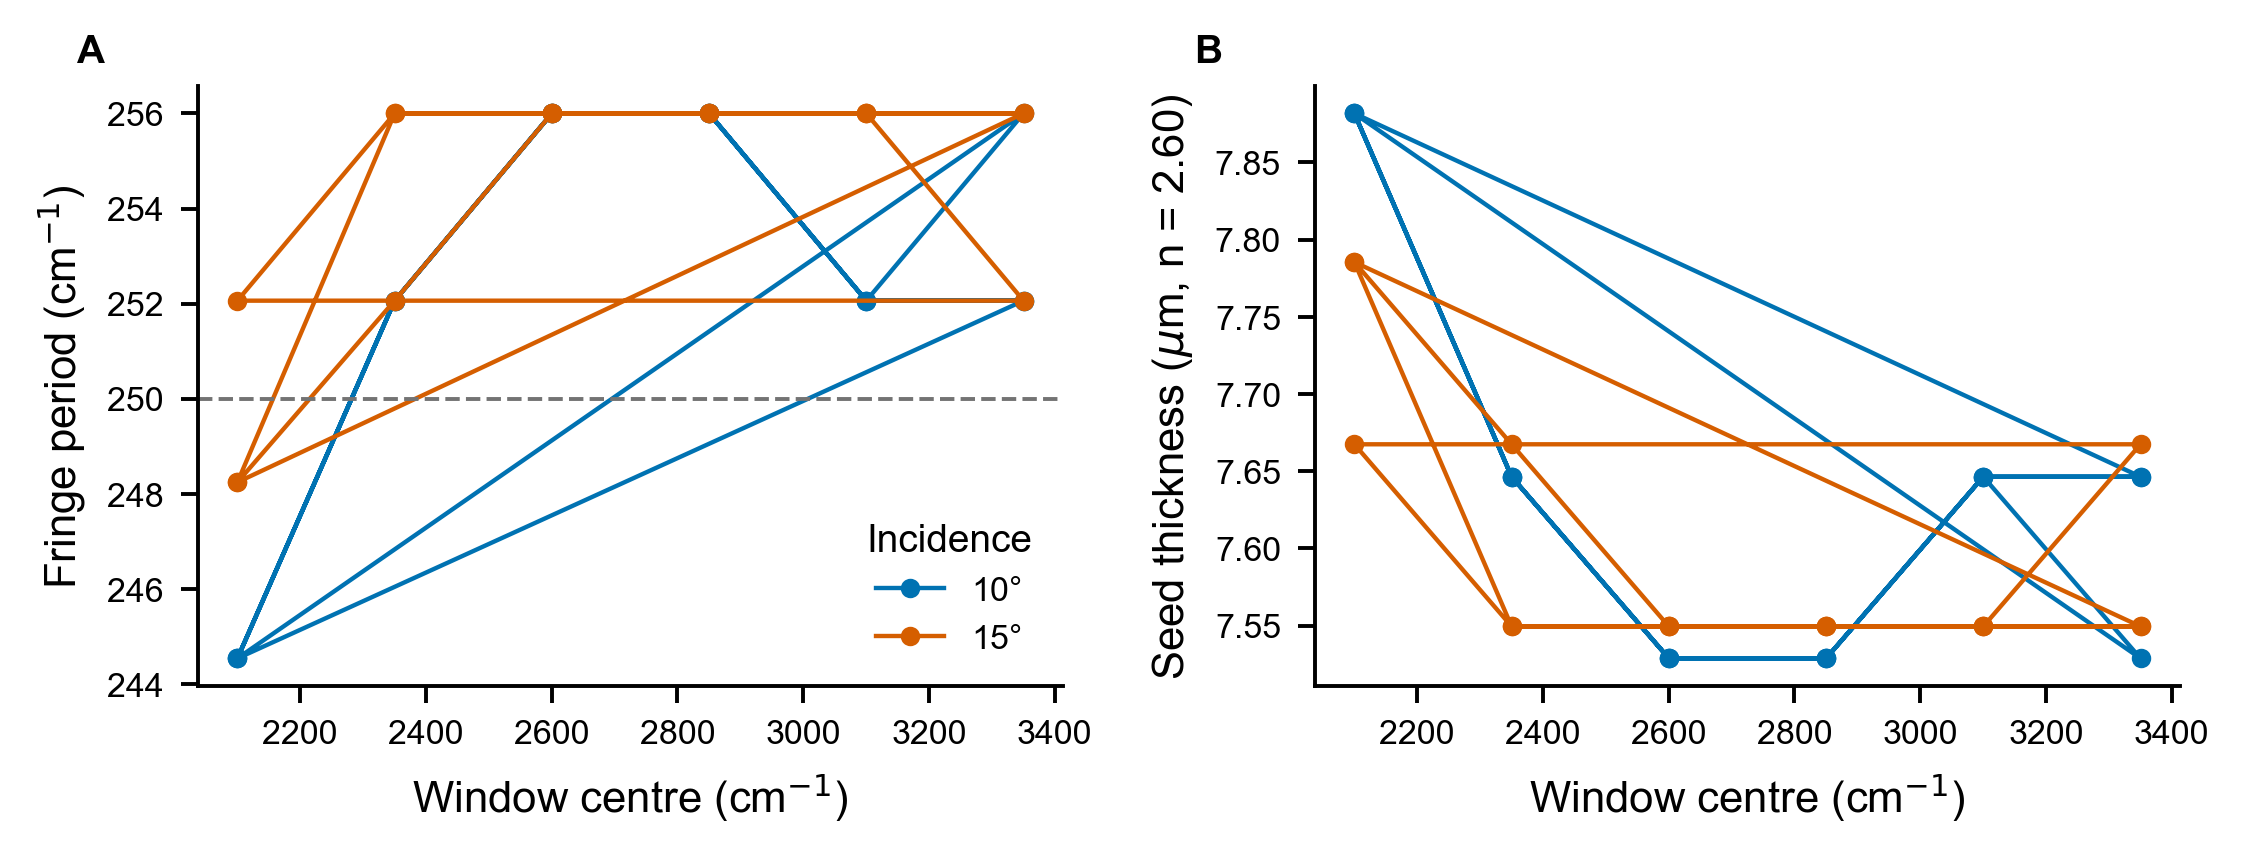
\includegraphics[width=.82\linewidth]{en_sliding_fft.png}
\caption{Sliding-window Fourier periods and their effective-index thickness seeds. The stability of the period supports the phase-scale observation; the seed remains convention dependent.}
\label{fig:sliding}
\end{figure}

\subsection{From phase scale to physical reflectance}
For a transparent effective-index approximation, a measured fringe period $\Delta\nu$ suggests
\begin{equation}
d_{\rm seed}\simeq\frac{10^4}{2n_{\rm eff}\cos\theta_1\Delta\nu},
\qquad \cos\theta_1=\left(1-\frac{\sin^2\theta_0}{n_{\rm eff}^2}\right)^{1/2}.
\label{eq:seed}
\end{equation}
Equation \ref{eq:seed} is useful for locating periodic basins, not for choosing among material conventions. With the observed period near $250\,\wn$, the project records approximately $6.5\,\um$, $7.7\,\um$ and $8.0\,\um$ under Larruquert, constant-$n=2.60$, and constrained-Dong index conventions respectively. This spread is itself evidence that a formula-only answer would be unjustified.

The primary model uses the phonon--Drude dielectric representation adapted from Dong et al. \cite{Dong2012},
\begin{equation}
\varepsilon(\nu)=\varepsilon_\infty\left[
\frac{\nu_L^2-\nu^2-i\Gamma_L\nu}{\nu_T^2-\nu^2-i\Gamma_T\nu}
-\frac{\nu_p^2}{\nu(\nu+i\gamma)}\right],\qquad \tilde n=\sqrt{\varepsilon}.
\label{eq:dielectric}
\end{equation}
Fresnel coefficients at the two interfaces and the phase $\beta=2\pi\tilde n d\cos\theta_1\nu 10^{-4}$ yield the Airy/transfer-matrix reflectance. The thickness $d$ is shared across angles. Material parameters are bounded nuisance variables; they are not claimed as electrical measurements of the wafer.

\subsection{Profiling instrument response}
An angle-specific scale and offset are necessary to avoid forcing modest measurement-chain differences into the physical parameters, but a flexible baseline could erase phase. We use the smallest useful response model,
\begin{equation}
y_a(\nu)=\alpha_aR_a(\nu;d,\eta)+b_a+e_a(\nu),
\end{equation}
and solve $(\alpha_a,b_a)$ by linear least squares for every trial $(d,\eta)$. The profiled objective is
\begin{equation}
\mathcal L_p(d,\eta)=\frac{1}{\sum_aN_a}\sum_a\min_{\alpha_a,b_a}
\sum_i[y_{a,i}-\alpha_aR_a(\nu_i;d,\eta)-b_a]^2+\Omega(\eta).
\label{eq:profile}
\end{equation}
This variable-projection step keeps calibration freedom visible rather than burying it in a high-dimensional nonlinear fit.

\section{Progressive baseline models and independent phase validation}
\subsection{Fringe spacing and FOD: from local extrema to multi-point regression}
For adjacent extrema of the same type, the interference order changes by approximately one. The round-trip optical path and Snell's law give
\begin{equation}
d\simeq\frac{10^4}{2n\cos\theta_1\Delta\nu},\qquad
\cos\theta_1=\sqrt{1-\left(\frac{\sin\theta_0}{n}\right)^2}.
\label{eq:spacing}
\end{equation}
Equation \eqref{eq:spacing} is a transparent baseline, but it uses only two extrema and treats refractive index and reflection phase as locally constant.

To reduce dependence on a single spacing, we use the fringe-order-difference (FOD) idea of Li \textit{et al.} \cite{Li2010}. For an extremum $\nu_i$ and reference extremum $\nu_{\rm ref}$, let $\Delta m_i$ denote the order difference and define
\begin{equation}
X_i=n\cos\theta_1(\nu_{\rm ref}-\nu_i),\qquad
\Delta m_i\simeq aX_i,\quad a=\frac{2d}{10^4}.
\end{equation}
The through-origin least-squares estimator, derived for the units and notation of this study, is
\begin{equation}
\hat d=5000\,\frac{\sum_iX_i\Delta m_i}{\sum_iX_i^2}.
\label{eq:fod}
\end{equation}
FOD is used as an interpretable multi-extremum seed, not as a replacement for full-spectrum modelling.

\paragraph{Baseline result and motivation for the next model.}
With constant $n=2.60$, FOD returns $7.191\pm0.148\,\um$ at $10^\circ$ and $6.603\pm0.089\,\um$ at $15^\circ$. The approximately $0.588\,\um$ separation shows that pooling extrema reduces local picking error but does not remove the systematic effect of a fixed refractive index. This result motivates dispersion correction rather than further tuning of extrema.

\subsection{Dispersive FOD and FFT: testing phase scale without over-calibration}
To expose refractive-index sensitivity, we replace the constant phase factor by
\begin{equation}
g(\nu)=n(\nu)\nu\cos\theta_1(\nu),\qquad
\Delta m_i\simeq\frac{2d}{10^4}\left[g(\nu_{\rm ref})-g(\nu_i)\right].
\label{eq:dispfod}
\end{equation}
The Larruquert optical-constant table is used here as a sensitivity input, not as a verified optical truth for the present specimen. The corresponding dispersive FOD estimates are $5.779\pm0.117\,\um$ and $5.292\pm0.065\,\um$. Their shift from constant-index FOD demonstrates that a more detailed formula cannot by itself solve a material-parameter mismatch.

As an independent periodicity check, the detrended spectrum is locally approximated as
\begin{equation}
R(\nu)\simeq B(\nu)+A(\nu)\cos\left[
\frac{4\pi d}{10^4}\sqrt{n_{\rm eff}^2-\sin^2\theta_0}\,\nu+\varphi\right].
\end{equation}
If FFT identifies a fringe period $\Delta\nu$, the study-derived seed is
\begin{equation}
d_{\rm FFT}=\frac{10^4}{2\Delta\nu\sqrt{n_{\rm eff}^2-\sin^2\theta_0}}.
\label{eq:fft}
\end{equation}
All detrending routes give a dominant period near $250\,\wn$, and sliding windows give $244.537$--$256.000\,\wn$. Thus the data contain a stable phase scale, but neither FFT nor FOD supplies a unique physical calibration. This is the reason to proceed to a full Airy/TMM model.

\begin{figure}[H]\centering
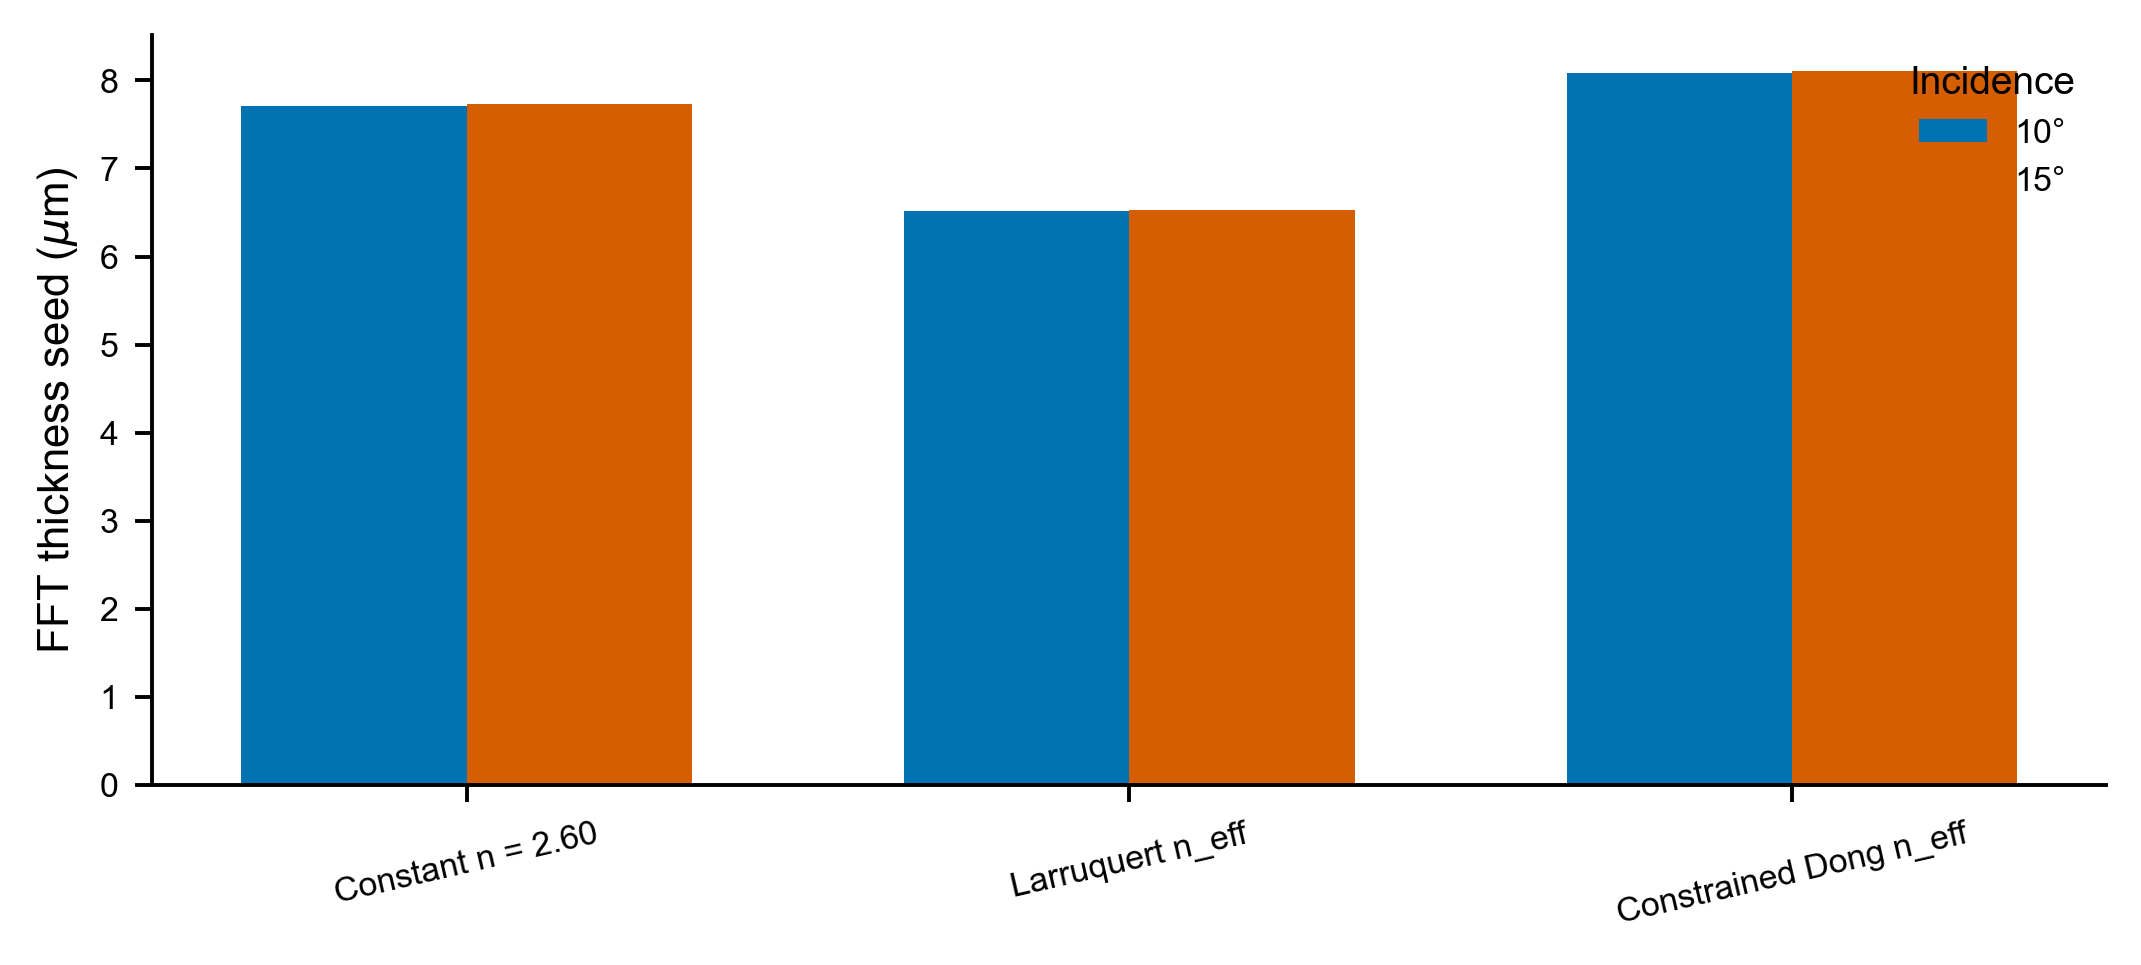
\includegraphics[width=.88\linewidth]{en_fft_thickness_seed.png}
\caption{FFT-derived thickness seeds under alternative preprocessing routes. Their common period supports a stable phase scale; the mapped thickness remains dependent on the effective-index convention.}\label{fig:fft}
\end{figure}

\section{Full-spectrum physical model and joint inference}
\subsection{Airy/TMM forward response and dielectric constraint}
FOD uses positions of extrema only, whereas full-spectrum inversion must also account for amplitude and multiple interface reflections. For the air--epilayer--substrate stack, the Airy/TMM form \cite{Troparevsky2010} is
\begin{equation}
r^q=\frac{r^q_{01}+r^q_{12}\exp(2{\rm i}\delta)}
{1+r^q_{01}r^q_{12}\exp(2{\rm i}\delta)},\quad
\delta=\frac{2\pi}{10^4}\tilde n_1(\nu)d\cos\theta_1\,\nu,
\end{equation}
\begin{equation}
R_{\rm model}=\frac{|r^s|^2+|r^p|^2}{2}.
\label{eq:tmm}
\end{equation}
The phonon--Drude dielectric response in Eq. \eqref{eq:dielectric} is adapted from Dong \textit{et al.} \cite{Dong2012}. The literature supplies the dielectric form; assigning separate epilayer and substrate scales, bounding them, and using them in a shared-thickness inversion are modelling choices of this study. In particular, $s_{\nu_p,\rm epi}\in[0.75,1.75]$ and $s_{\nu_p,\rm sub}\in[0.75,1.25]$ are physical regularisation bounds, not carrier measurements.

\subsection{Shared thickness, candidate basins and profiled joint objective}
FFT/FOD candidates are refined through coordinate search and bounded local optimisation under Eq. \eqref{eq:profile}; the two angles must share one thickness. Under the Dong2012 Table-2 dielectric state, the single-angle minima occur near $7.460\,\um$ at $10^\circ$ and $7.400\,\um$ at $15^\circ$. Their closer agreement than the FOD values indicates that complex index and multiple reflections explain part of the mismatch left by the baseline models. With shared thickness, profiled affine terms and the plasma bounds, local refinement yields $d^*=7.465\,\um$ and joint RMSE $0.00171152$, improving the initial coordinate-search value ($d=7.455\,\um$, RMSE $0.00173772$) by 1.508\%. This internal improvement is not presented as external accuracy.

\section{Measurement workflow}
The workflow begins with centring, moving-average, polynomial, rolling baseline and first-difference preprocessing. Dominant FFT peaks, sliding FFT windows and same-type-extremum FOD relations generate candidate basins. They are not averaged into a final number. Each candidate is evaluated under the same two-angle optical objective, with a common thickness and bounded dielectric parameters. Finally, the interpretation is challenged by a thickness profile, moving-block resampling of correlated residuals, four spectral-weight rules, per-angle residual inspection and parameter-bound checks. This order follows the logic of measurement: a fringe must first be observed, then physically mapped, then stress-tested.

\section{Results}
\subsection{Headline thickness statement}
Taken together, the recorded results support a \textbf{7.4--7.6 \um} candidate interval for the SiC epitaxial layer. The constrained dual-angle inversion locates a representative value at $d^*=7.465\,\um$. The interval, rather than the third decimal place of $d^*$, is the primary result because the model does not fully close across angles and has no independent thickness reference.

\subsection{Phase evidence and the need for a full model}
All preprocessing routes produce a dominant full-band period close to $250\,\wn$; sliding windows span $244.537$--$256.000\,\wn$. The fringe pattern is therefore not a smoothing artefact. Nevertheless, constant-index FOD gives $7.191\pm0.148\,\um$ at $10^\circ$ and $6.603\pm0.089\,\um$ at $15^\circ$, while dispersive Larruquert FOD gives $5.779\pm0.117\,\um$ and $5.292\pm0.065\,\um$. These simplified routes agree on the presence of phase but not on the thickness calibration. This is why their role is candidate generation rather than final adjudication.

\subsection{Constrained two-angle fit and local robustness}
Using the Dong-type optical state, single-angle searches first locate minima near $7.460\,\um$ ($10^\circ$) and $7.400\,\um$ ($15^\circ$). The shared-thickness refinement gives $d^*=7.465\,\um$, joint RMSE $0.00171152$, compared with an initial coordinate-search value of $7.455\,\um$ and RMSE $0.00173772$. The numerical improvement is modest (1.508\%) and is reported as such; it does not create external validation.

\begin{figure}[H]\centering
\begin{minipage}{.48\linewidth}\centering
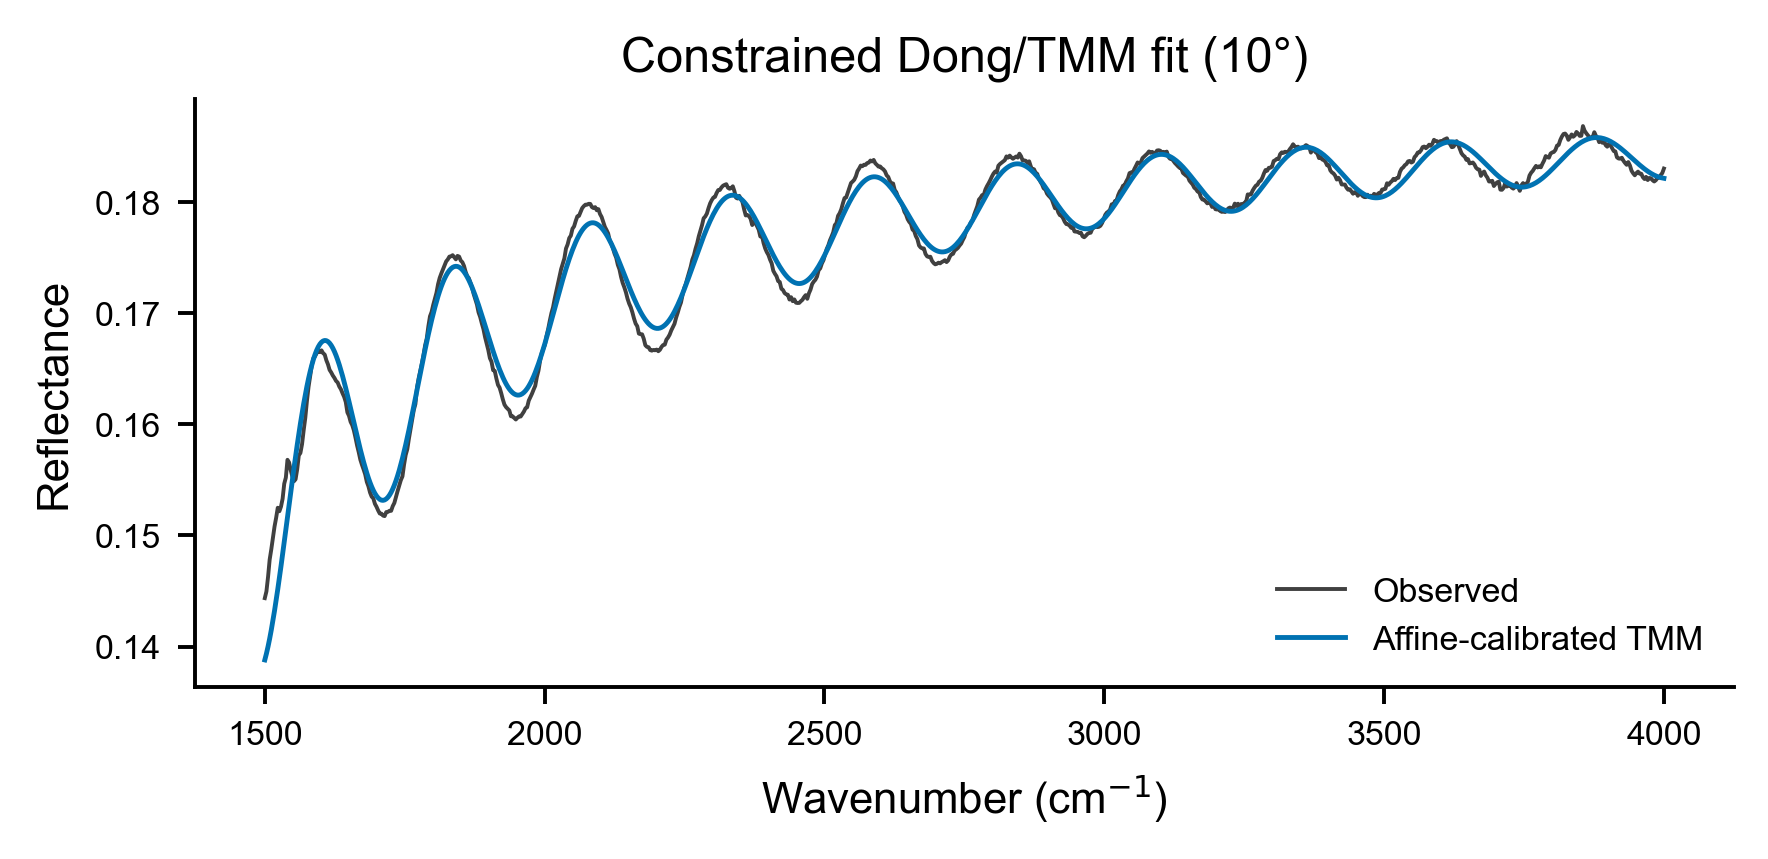
\includegraphics[width=\linewidth]{en_tmm_fit_10deg.png}\\[-1mm]\small (a) $10^\circ$
\end{minipage}\hfill
\begin{minipage}{.48\linewidth}\centering
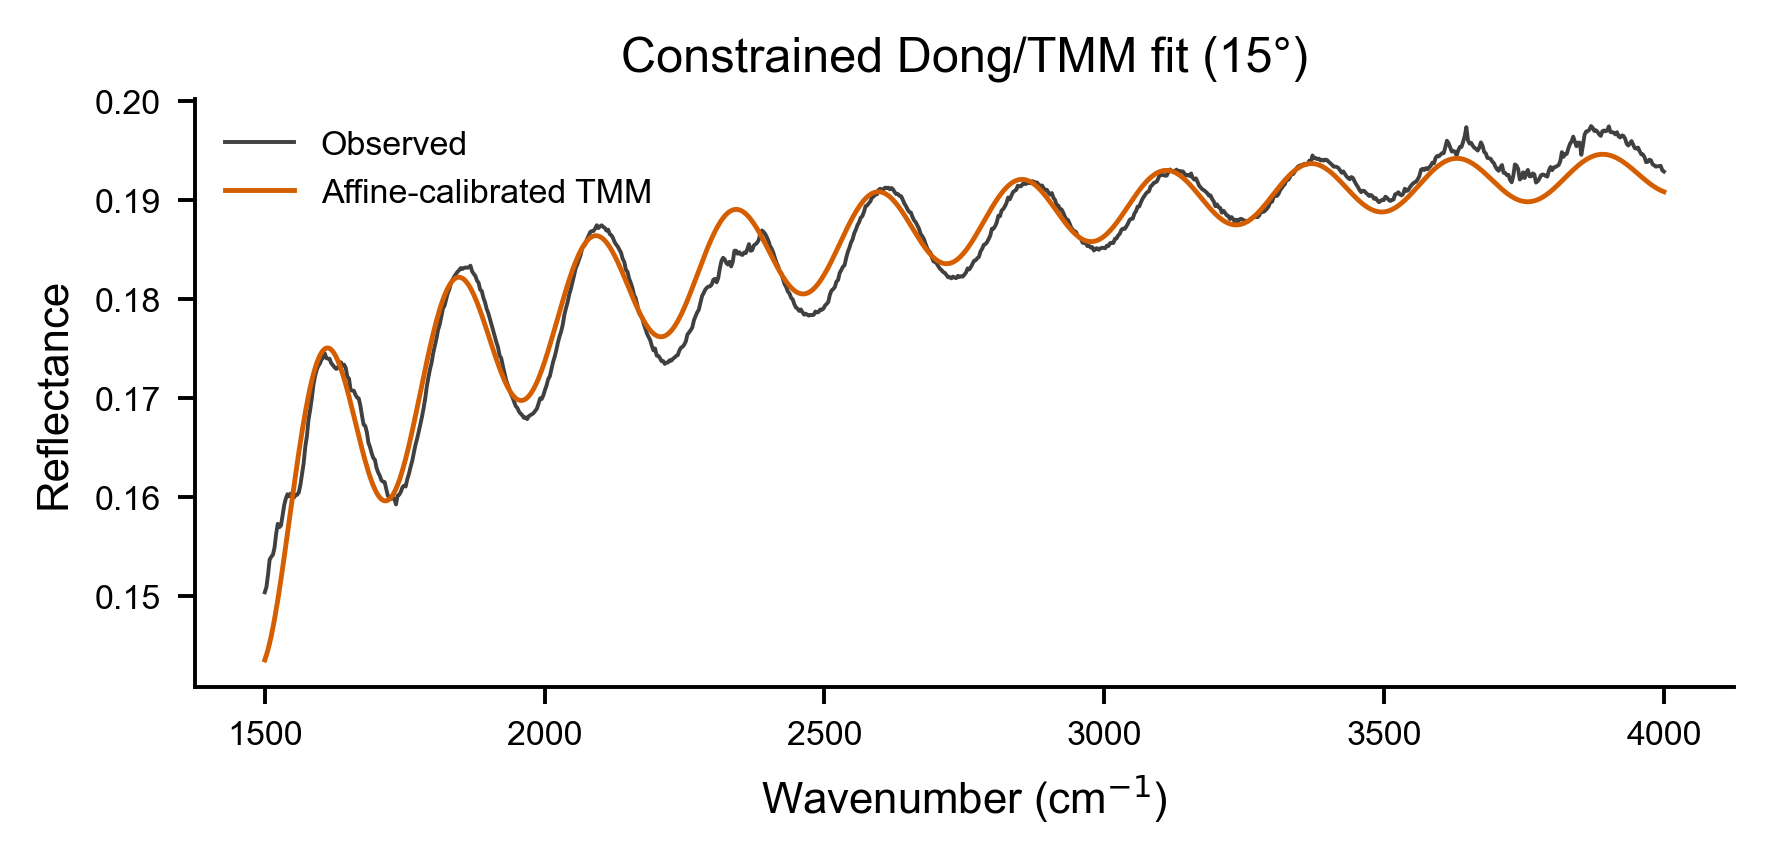
\includegraphics[width=\linewidth]{en_tmm_fit_15deg.png}\\[-1mm]\small (b) $15^\circ$
\end{minipage}
\caption{Representative constrained Dong/TMM fits. The shared-thickness test must be read together with the structured residuals in Fig.~\ref{fig:residual}.}\label{fig:tmmfit}
\end{figure}

\begin{table}[H]\centering\small
\caption{Evidence hierarchy for the reported thickness.}\label{tab:evidence}
\begin{tabular}{p{.34\linewidth}p{.24\linewidth}p{.31\linewidth}}\toprule
Evidence & Recorded result & Permitted interpretation\\\midrule
Multi-route FFT & $\Delta\nu\approx250\,\wn$; $244.537$--$256.000\,\wn$ sliding range & Stable interference phase scale.\\
Shared constrained TMM & $d^*=7.465\,\um$; RMSE 0.00171152 & Representative value under this optical model.\\
Band-weight perturbation & $7.465$--$7.485\,\um$ & Local valley is not selected by one weighting rule.\\
Fixed-material checks & 5\% support $7.435$--$7.475\,\um$; bootstrap $7.44488$--$7.46512\,\um$ & Conditional stability, not total uncertainty.\\
Residual audit & RMSE 0.00131074/0.00211230; lag-one 0.9726/0.9834 & Model/material explanation remains incomplete.\\\bottomrule
\end{tabular}
\end{table}

Equal, FFT-selected, FFT-downweighted and continuous-weight objectives attain minima of $7.465$, $7.485$, $7.475$ and $7.470\,\um$, respectively: a maximum displacement of $0.020\,\um$. At fixed material state, the 5\% profile support is $7.435$--$7.475\,\um$; 120 moving-block residual bootstrap replicates have 2.5--97.5\% quantiles of $7.44488$--$7.46512\,\um$. These are useful tests of stability against the recorded residual structure, but they deliberately do not propagate uncertainty in dispersion, incidence angle, model form or dielectric priors.

\begin{figure}[H]\centering
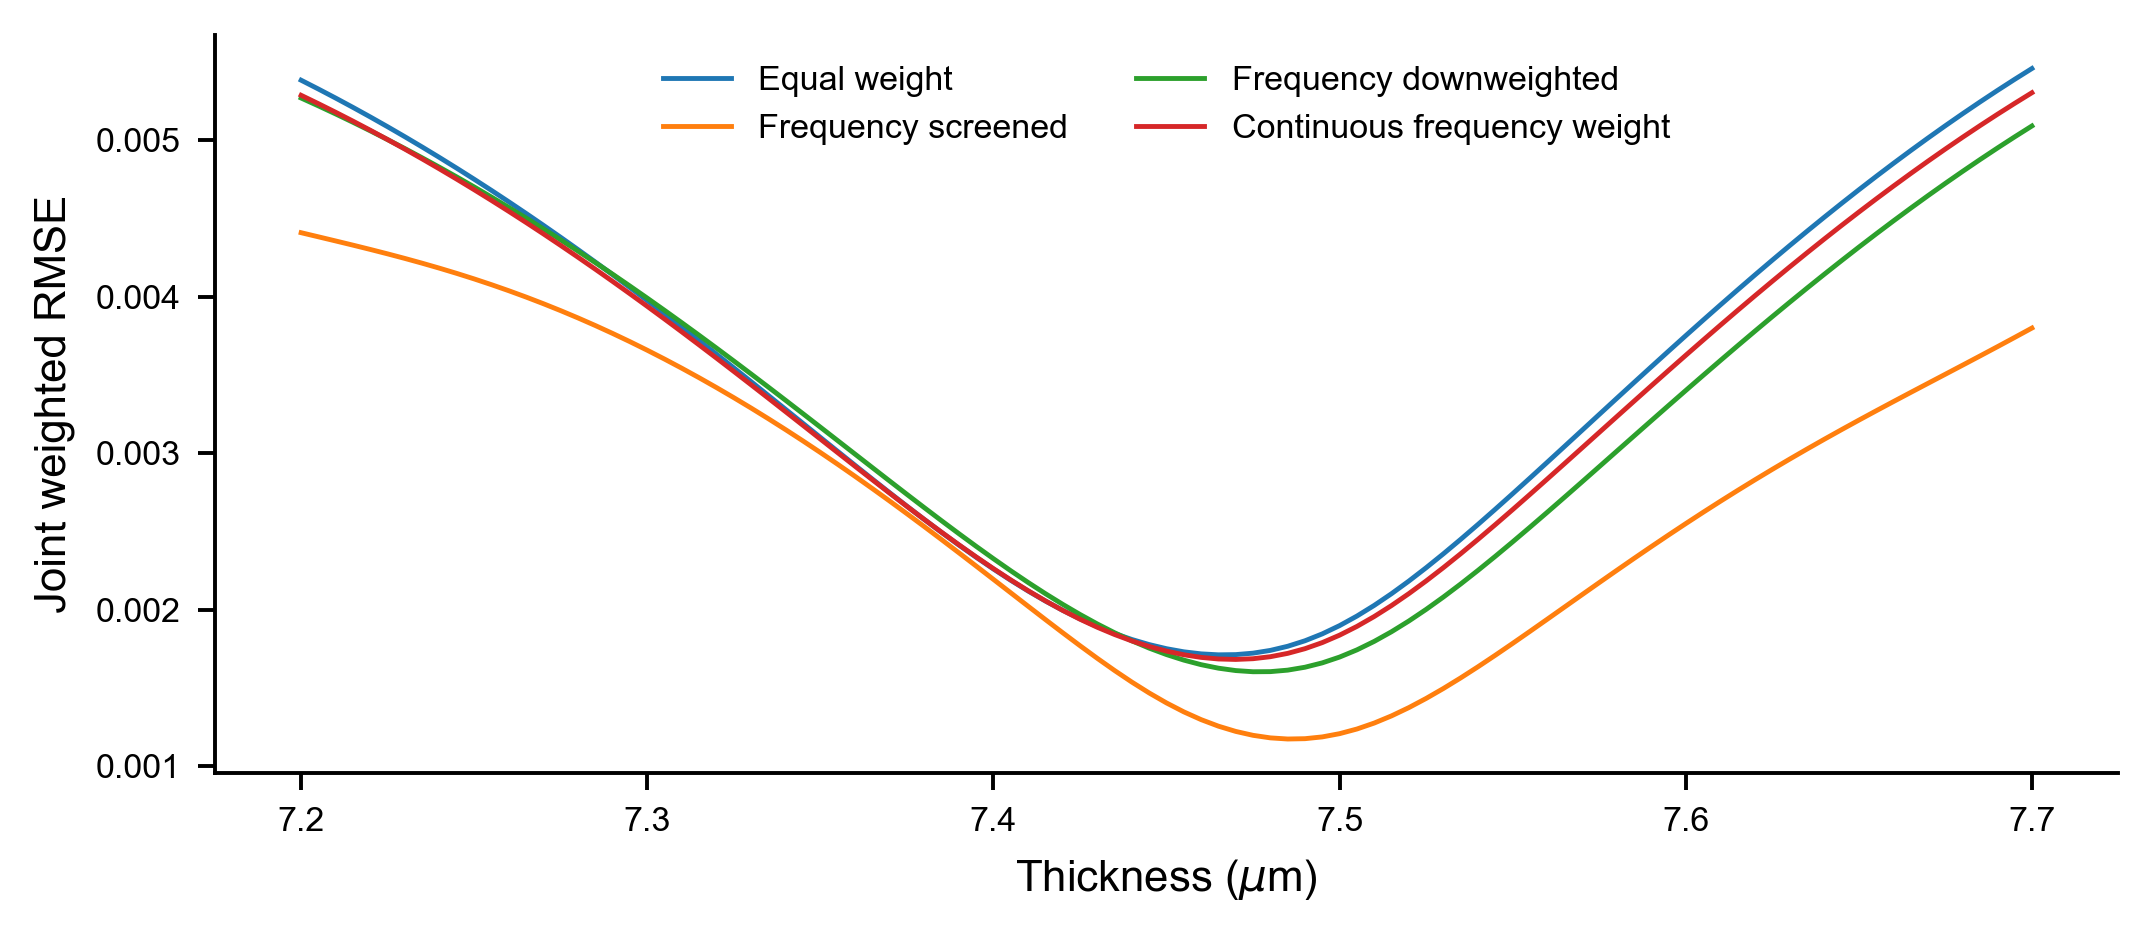
\includegraphics[width=.84\linewidth]{en_band_weighted_profile.png}
\caption{Thickness profiles under four band-weight specifications. The close minima are a robustness check against selected spectral regions, not a full physical confidence interval.}\label{fig:weights}
\end{figure}

\begin{figure}[H]\centering
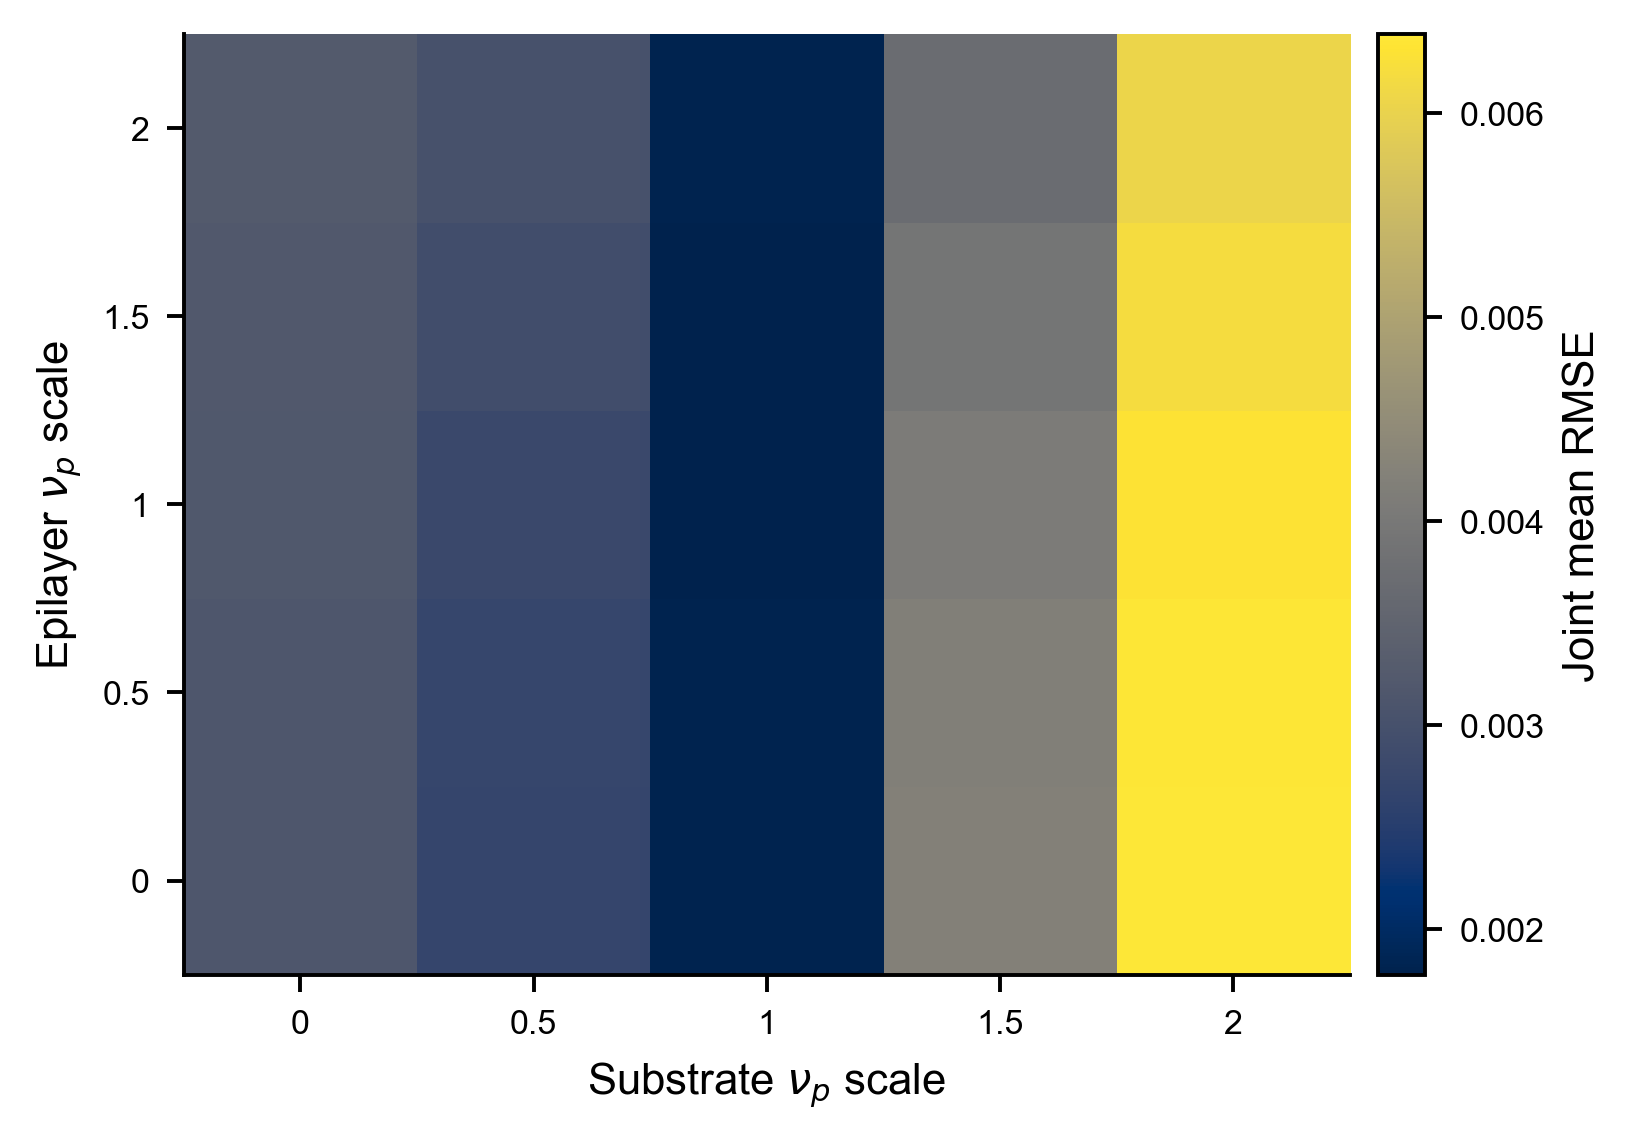
\includegraphics[width=.82\linewidth]{en_nup_rmse_heatmap.png}
\caption{Joint-RMSE landscape under plasma-frequency scaling. A persistent thickness basin is visible, while sensitivity to material parameters remains part of the claim boundary.}\label{fig:nup}
\end{figure}

\subsection{Counter-evidence that sets the claim boundary}
The per-angle residuals are not exchangeable. Their RMSE values are 0.00131074 at $10^\circ$ and 0.00211230 at $15^\circ$, with lag-one autocorrelations of 0.9726 and 0.9834. The $15^\circ$ mismatch is especially persistent in the $1500$--$2500\,\wn$ and $3500$--$4000\,\wn$ bands. In addition, the epitaxial plasma-scale parameter reaches its upper bound of 1.75. These observations do not invalidate the local thickness valley, but they preclude interpreting the fit as a complete physical account of the spectra.

\begin{figure}[H]\centering
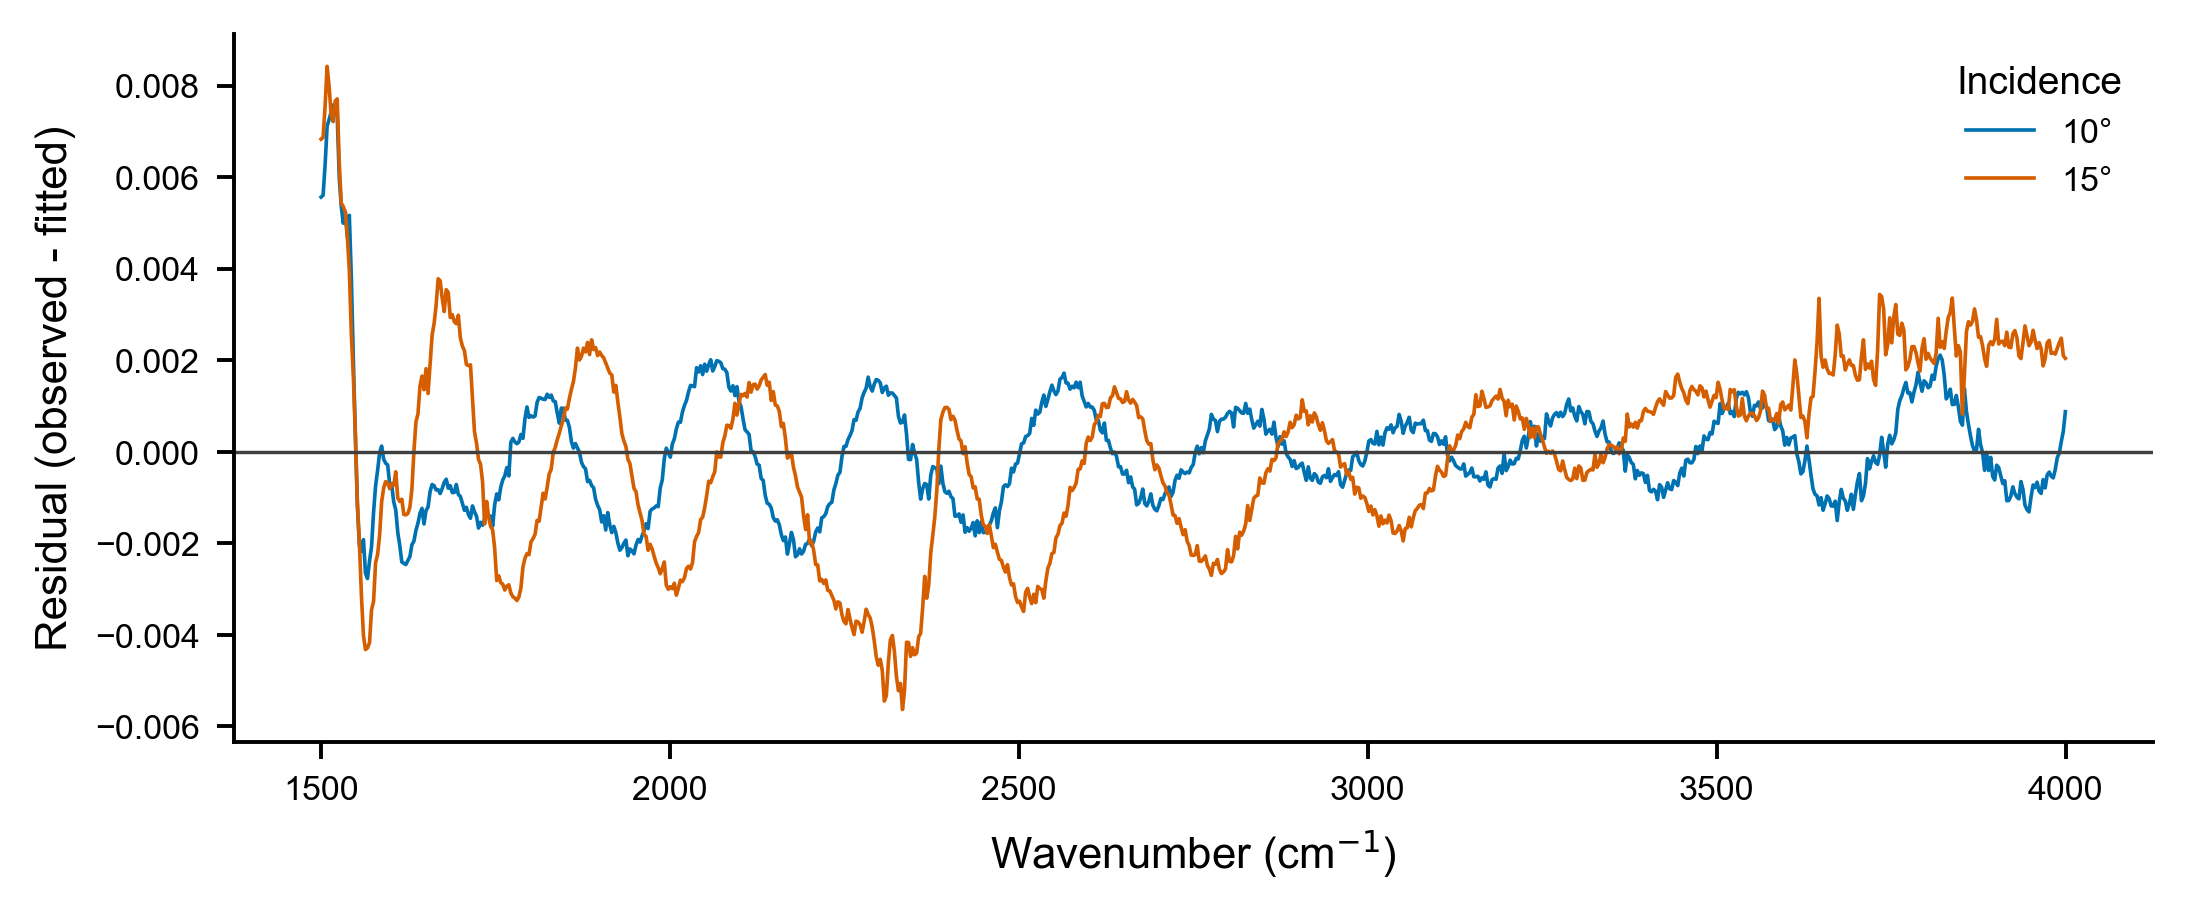
\includegraphics[width=.88\linewidth]{en_residual_diagnostics.png}
\caption{Angle-specific residual diagnostics. Structured residuals, particularly at $15^\circ$, prevent an RMSE-only interpretation of the fit.}\label{fig:residual}
\end{figure}

\section{Final evidence audit, result summary and model appraisal}
The final statement should not depend on a collection of disconnected scripts or a single tuning run. We therefore audit only recorded experiments on a common thickness axis: no parameter is retuned, the search is not enlarged, and FFT/FOD seeds are not elevated to final thickness evidence. The two-angle Dong2012/TMM calculations cover $7.400$--$7.460\,\um$; plasma-frequency sensitivity retains $7.440$--$7.580\,\um$; damping, phonon, band, constrained-refinement, fixed-material profile, moving-block bootstrap and weight-profile checks do not displace the valley outside $7.4$--$7.6\,\um$. The audited strong-evidence coverage is consequently $7.400$--$7.580\,\um$, reported conservatively as $7.4$--$7.6\,\um$ rather than as an unconditional confidence interval.

\begin{figure}[H]\centering
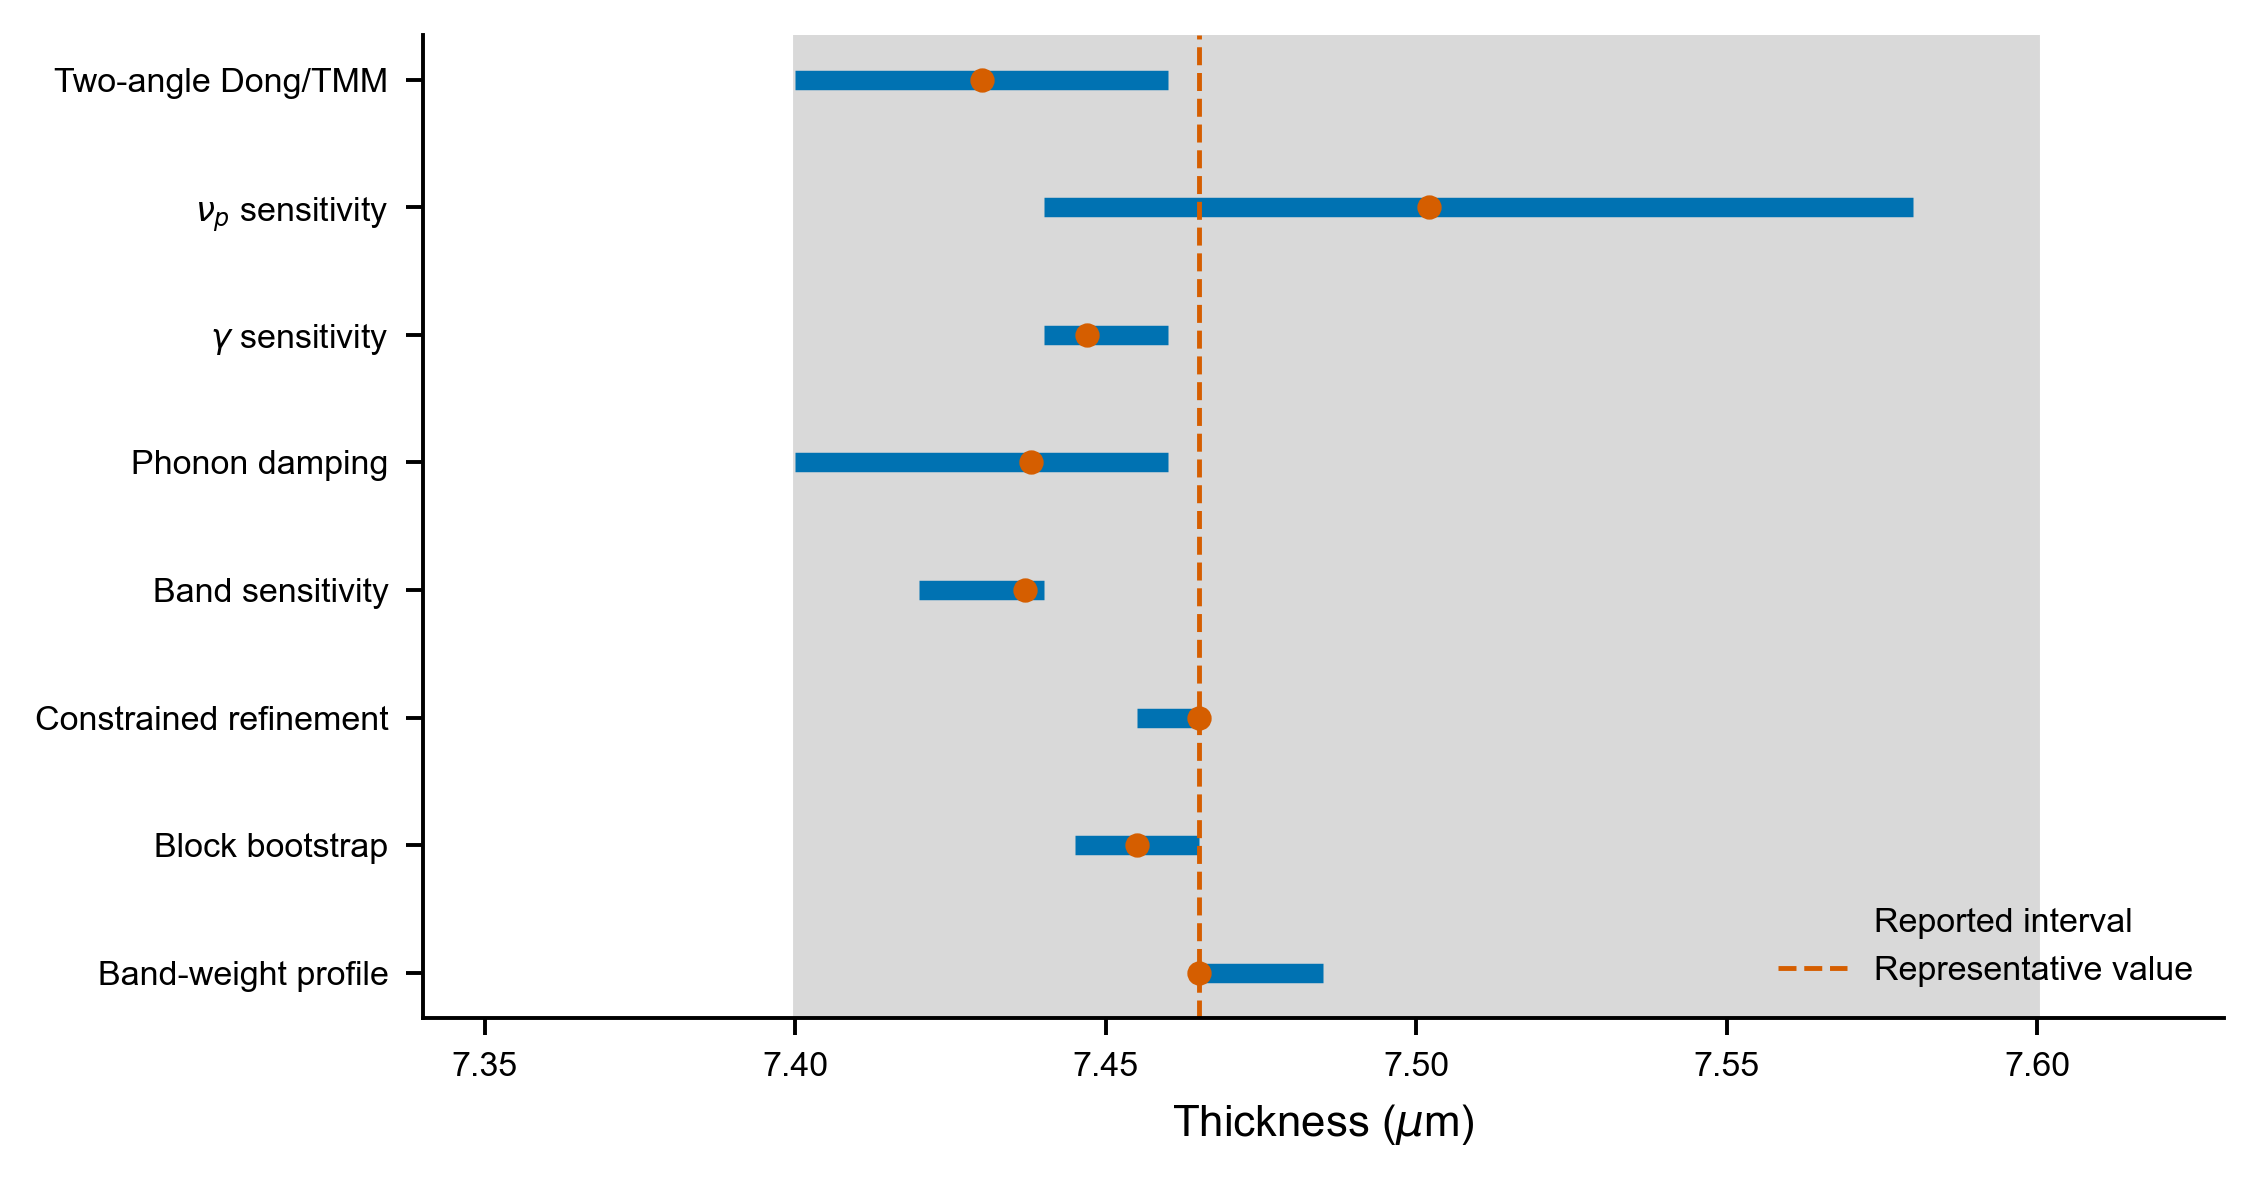
\includegraphics[width=.90\linewidth]{en_final_evidence_audit.png}
\caption{Final evidence-consistency audit. Each bar represents a recorded experiment on the common thickness axis; conditional ranges are not combined into a physical confidence interval.}\label{fig:finalaudit}
\end{figure}

\begin{table}[H]\centering\small
\caption{Integrated result summary.}\label{tab:summary}
\begin{tabular}{p{.35\linewidth}p{.24\linewidth}p{.30\linewidth}}\toprule
Quantity & Recorded result & Permitted interpretation\\\midrule
FFT/sliding period & $250\,\wn$; $244.537$--$256.000\,\wn$ & Stable phase scale, not unique calibration\\
Two-angle Dong/TMM & $7.460/7.400\,\um$ & Full-spectrum estimates that do not fully close\\
Constrained joint solution & $7.465\,\um$; RMSE 0.00171152 & Representative local model value\\
$\nu_p$ sensitivity & $7.440$--$7.580\,\um$ & Principal material-perturbation basin\\
Profile/bootstrap & $7.435$--$7.475\,\um$; $7.44488$--$7.46512\,\um$ & Conditional local stability\\
Final audit & $7.400$--$7.580\,\um$ & Recorded strong-evidence coverage\\
Reported interval & \textbf{7.4--7.6 $\um$} & Most defensible measurement statement\\\bottomrule
\end{tabular}
\end{table}

The framework is strong because it orders the evidence: stable periodicity, transparent baselines, bounded full-spectrum physics, then targeted robustness and residual tests. Its limitation is equally material: Dong2012 parameters are transferred from a literature sample, damping bounds are incomplete, the epitaxial plasma scale reaches a boundary, and the $15^\circ$ residual is structured. Independent metrology, verified angle/polarisation conditions and traceable material priors are therefore more useful next steps than adding unconstrained fitting freedom.

\section{Discussion and conclusion}
The measurement result is stronger than a single fringe-spacing calculation because it survives two acquisition angles, an explicit complex-index model, constrained sharing of thickness, nuisance-term profiling and targeted perturbations. It is weaker than a calibrated metrology result because its internal consistency is conditional on the optical model. The correct interpretation is consequently asymmetric: the data make $7.4$--$7.6\,\um$ a well-supported candidate range for this wafer; they do not establish a certified absolute thickness, an error percentage, or a general-purpose carrier extraction.

The next experiment should break the remaining ambiguity rather than merely tune the optimizer. An independent profilometer, cross-sectional SEM or ellipsometric measurement would permit an accuracy comparison. Polarisation-resolved measurements, a verified angle calibration and independently constrained optical/carrier priors would test whether the structured $15^\circ$ residual arises from material anisotropy, angle error, or an inadequate dielectric response. Until those tests are available, $7.465\,\um$ should remain a representative constrained-model value inside the reported $7.4$--$7.6\,\um$ measurement interval.

\section*{Data and code availability}
The source workbooks, analysis scripts and recorded outputs used for this paper are retained in the associated project archive. No external thickness label or unrecorded experimental parameter was introduced in the analysis.

\section*{Use of references in the model}
Li et al. \cite{Li2010} supply the FOD method premise; Dong et al. \cite{Dong2012} supply the 4H--SiC Lorentz--Drude dielectric constraint; and Troparevsky et al. \cite{Troparevsky2010} supply the Airy/transfer-matrix formalism. These sources support the model form and its physical constraints, not an external ground-truth thickness or an accuracy validation for this wafer.

\begin{thebibliography}{9}
\bibitem{Li2010} Z.-Y. Li, J.-W. Sun, Y.-M. Zhang, Y.-M. Zhang and X.-Y. Tang. Methods for Thickness Determination of SiC Homoepilayers by Using Infrared Reflectance Spectroscopy. \emph{Chinese Physics Letters} \textbf{27}, 068103 (2010). doi:10.1088/0256-307x/27/6/068103.
\bibitem{Tang2009} X. Tang, Y. Zhang, Z. Li, Y. Zhang and H. Yao. Thickness determination of 4H-SiC epitaxial films by infrared reflectance. \emph{2009 IEEE International Conference of Electron Devices and Solid-State Circuits}, 295--297 (2009). doi:10.1109/edssc.2009.5394259.
\bibitem{Dong2012} L. Dong et al. Characterization of 4H--SiC substrates and epilayers by Fourier transform infrared reflectance spectroscopy. \emph{Chinese Physics B} \textbf{21}, 047802 (2012). doi:10.1088/1674-1056/21/4/047802.
\bibitem{Troparevsky2010} M. C. Troparevsky, A. S. Sabau, A. R. Lupini and Z. Zhang. Transfer-matrix formalism for the calculation of optical response in multilayer systems: from coherent to incoherent interference. \emph{Optics Express} \textbf{18}, 24715 (2010). doi:10.1364/oe.18.024715.
\end{thebibliography}
\end{document}
